\begin{figure}[h!]
	\center
	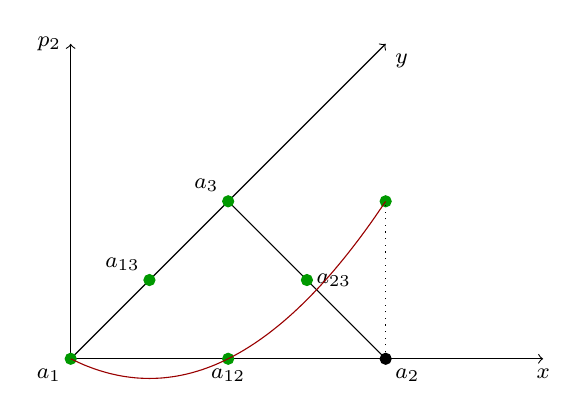
\begin{tikzpicture}[scale=2]

	\pgfmathsetmacro{\zerox}{0}
	\pgfmathsetmacro{\zeroy}{0}
	
	\pgfmathsetmacro{\ax}{\zerox + 2}
	\pgfmathsetmacro{\ay}{\zeroy + 1}
	
	
	% triangle
	\draw (\zerox,\zeroy) ++(2,0)-- ++(-1,1) --cycle;
	
	%axis
	\draw[->] (\zerox,\zeroy) -- ++(3,0);
	\draw[->] (\zerox,\zeroy) -- ++(0,2);
	\draw[->] (\zerox,\zeroy)  -- ++(2,2);
	\fill[black,font=\footnotesize] (\zerox,\zeroy) ++(3,0) node[below] {$x$}
									(\zerox,\zeroy) ++(2,2) node[below right] {$y$}
									(\zerox,\zeroy) ++(0,2) node[left] {$p_2$};
	
	% dots for a_2
	\filldraw (\zerox,\zeroy) ++(\ax,0) circle (1pt);
	\filldraw[green!60!black] (\ax,\ay) circle (1pt);
	\draw[dotted] (\zerox,\zeroy) ++(\ax,0)-- ++(0,\ay);
	
	% dots for a_i, a_{ij}
	\filldraw[green!60!black] (\zerox,\zeroy) circle (1pt);
	\filldraw[green!60!black] (\zerox,\zeroy) ++(1,1) circle (1pt);
	\filldraw[green!60!black] (\zerox,\zeroy) ++(1,0) circle (1pt);
	\filldraw[green!60!black] (\zerox,\zeroy) ++(0.5,0.5) circle (1pt);
	\filldraw[green!60!black] (\zerox,\zeroy) ++(1.5,0.5) circle (1pt);
	% nodes for for a_i, a_{ij}
	\fill[black,font=\footnotesize] (\zerox,\zeroy) node[below left] {$a_1$}
									(\zerox,\zeroy) ++(2,0) node[below right] {$a_2$}
									(\zerox,\zeroy) ++(1,1) node[above left] {$a_3$}
									(\zerox,\zeroy) ++(1,0) node[below] {$a_{12}$}
									(\zerox,\zeroy) ++(0.5,0.5) node[above left] {$a_{13}$}
									(\zerox,\zeroy) ++(1.5,0.5) node[right] {$a_{23}$};
	% linear parts
	%\draw[green!60!black] (\ax,\ay) -- ++(-1,-1.2); % line (a_2,1) to (a_12,0)
	%\draw[green!60!black] (\ax,\ay) -- ++(-0.5,-0.7); % line (a_2,1) to (a_23,0)
	%\draw[green!60!black] (\ax,\ay) -- ++(-0.75,-0.95); % line (a_2,1) to ???
	
	\draw[scale=2,domain=0:1,smooth,variable=\x,red!60!black] plot ({\x},{1/2*\x*(2*\x-1)});

	\end{tikzpicture}
		
	\caption{quadratic basisfunction $p_2$}
	\label{ch1_quadratic_basisfunction}

\end{figure}